\documentclass[cacheSimReport.tex]{subfiles}
\begin{document}

\section*{\textsc{\Large Results and Discussion}}

The first valuable metric is a comparison of the execution times between the different traces as well as the different configurations.

\smallskip

\hspace{-.9cm}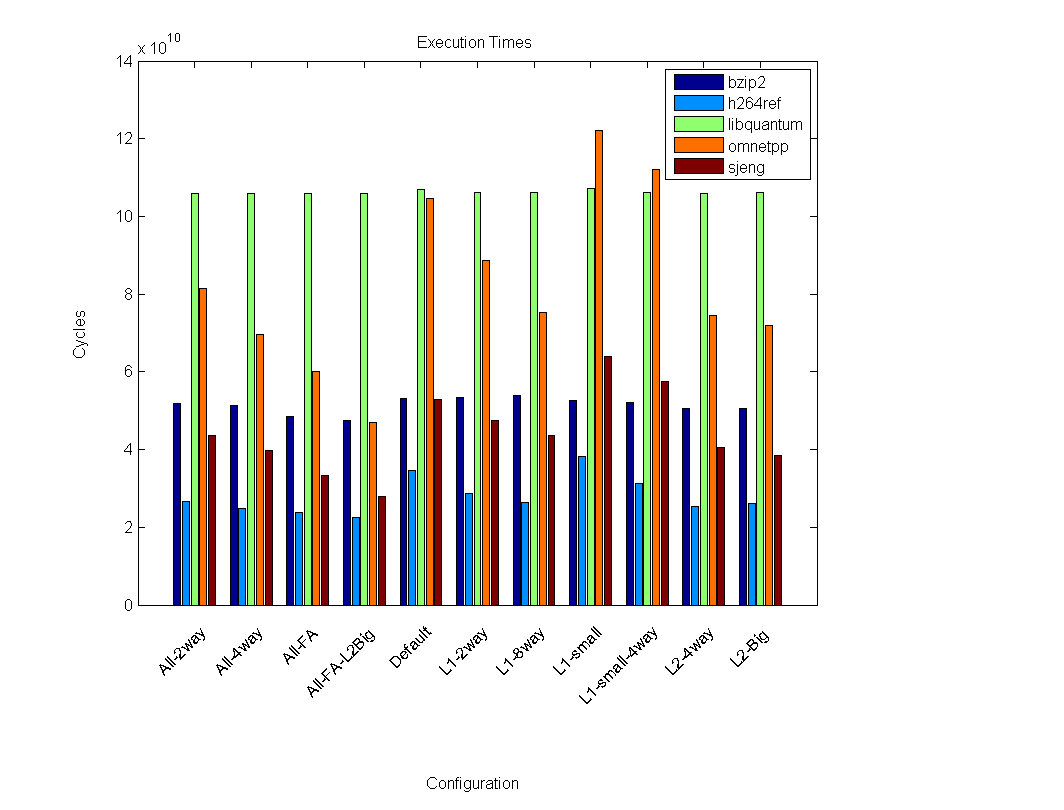
\includegraphics{executionTime.png}

\pagebreak

In this figure the columns of the bar chart are organized first by the configuration run, then the trace. Excepting the libquantum trace, the traces follow a regular pattern. The execution times go from smallest with the All-FA-L2Big configuration to the largest execution time L1-small. The amount of variation for different traces also differs greatly. Libquantum and bzip2 have a relatively small amount of variation between different configs, while omnetpp varies wildly. This behavior is likely due to the types of instructions contined within the trace. The omnetpp trace, for example, gains large benifits from increasing the associativity of both the L1 and L2 cache, as well as benefit from increasing the size of the L2 cache. The libquantum trace acts in a different fashion, not seeming to gain benefit from any sort of modifications made to the cache structure. Though libquatum was the smallest trace size at 4.2GB, it took the most cycles to run in 9 of the 11 configurations this is likely due to its hit rate which will be discussed later in this section.

\smallspace

The next five images show comparisons of the hit rates for the L1 caches and the L2 cache for each of the different configurations with each of the five traces. This data sheds light on the results in the previous section.

\hspace{-.9cm}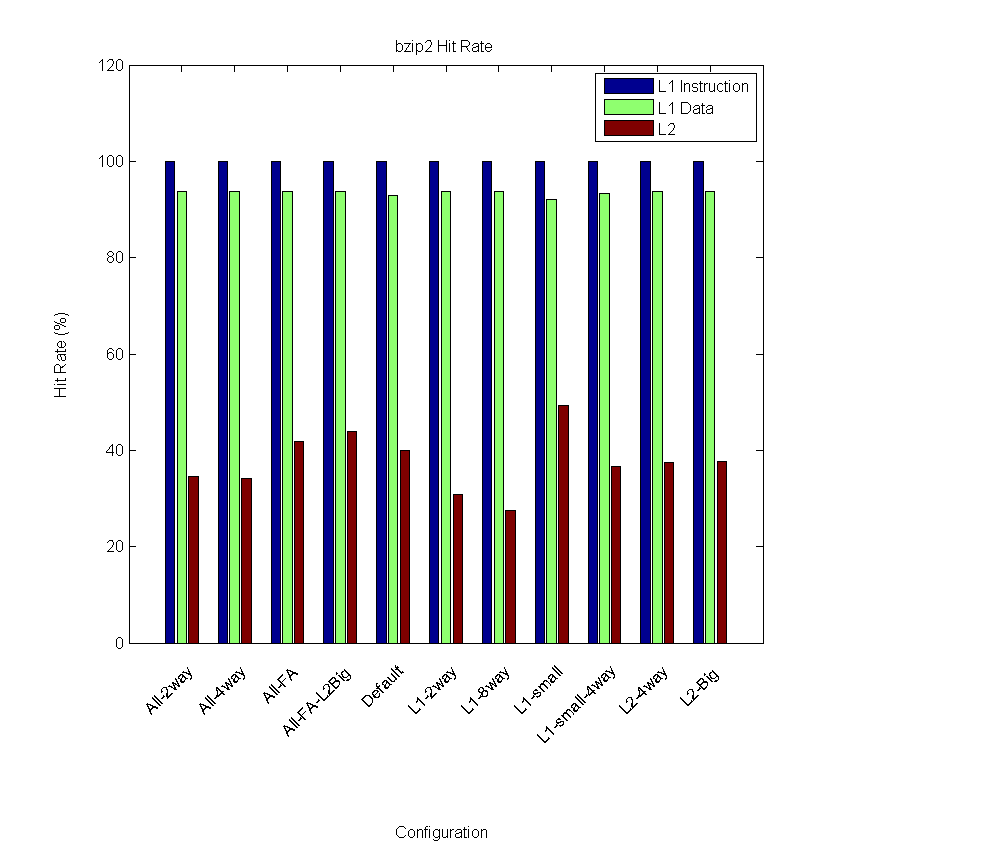
\includegraphics{hitRate_bzip2.png}

The hit rate results are different for the bzip2 trace as they have by far the lowest L2 cache hit rate at every configuration. The L1 instruction hit rate is near 100\% while the L2 data hit rate hovers at around 93\%. These relatively good hit rates keep the run time on the low side, but the under 50\% L2 hit rate takes a toll on overall performance.

\hspace{-.9cm}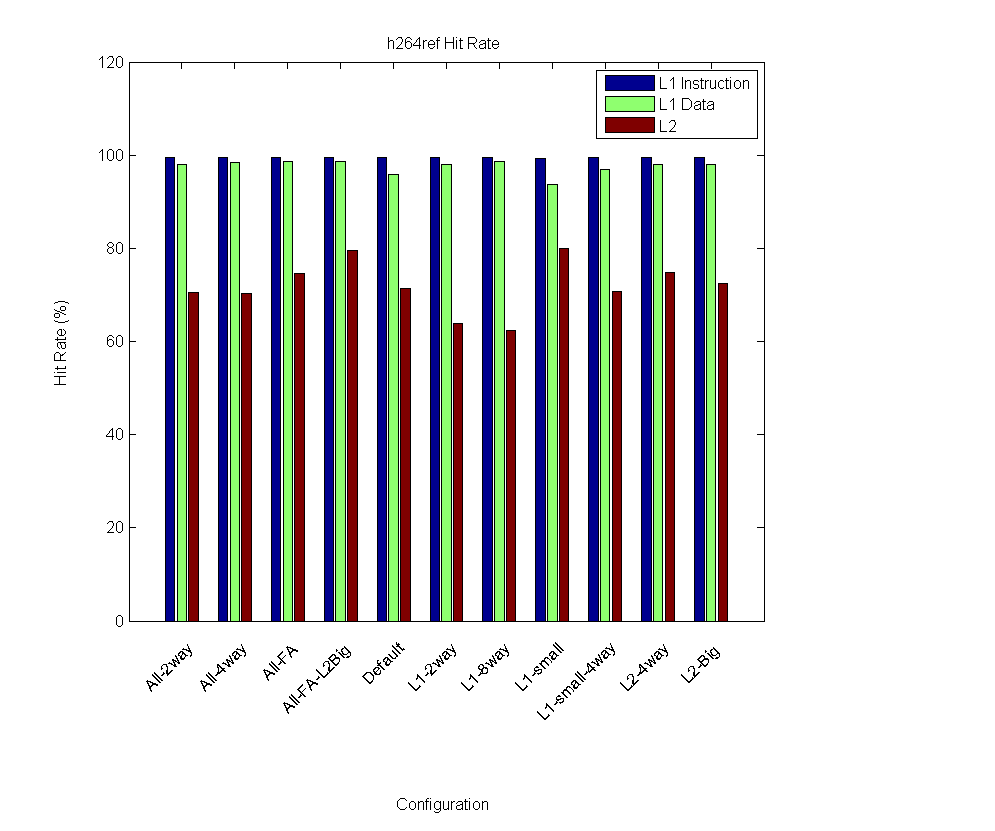
\includegraphics{hitRate_h264ref.png}

\hspace{-.9cm}\includegraphics{hitrate_libquantum.png}

\hspace{-.9cm}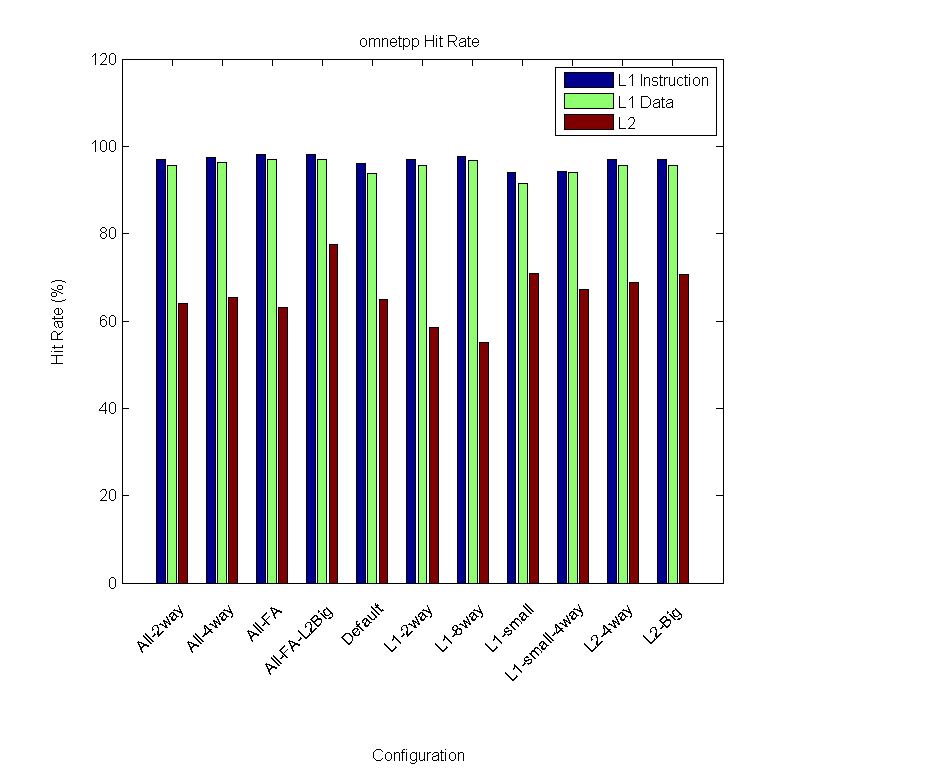
\includegraphics{hitRate_omnetpp.png}

\hspace{-.9cm}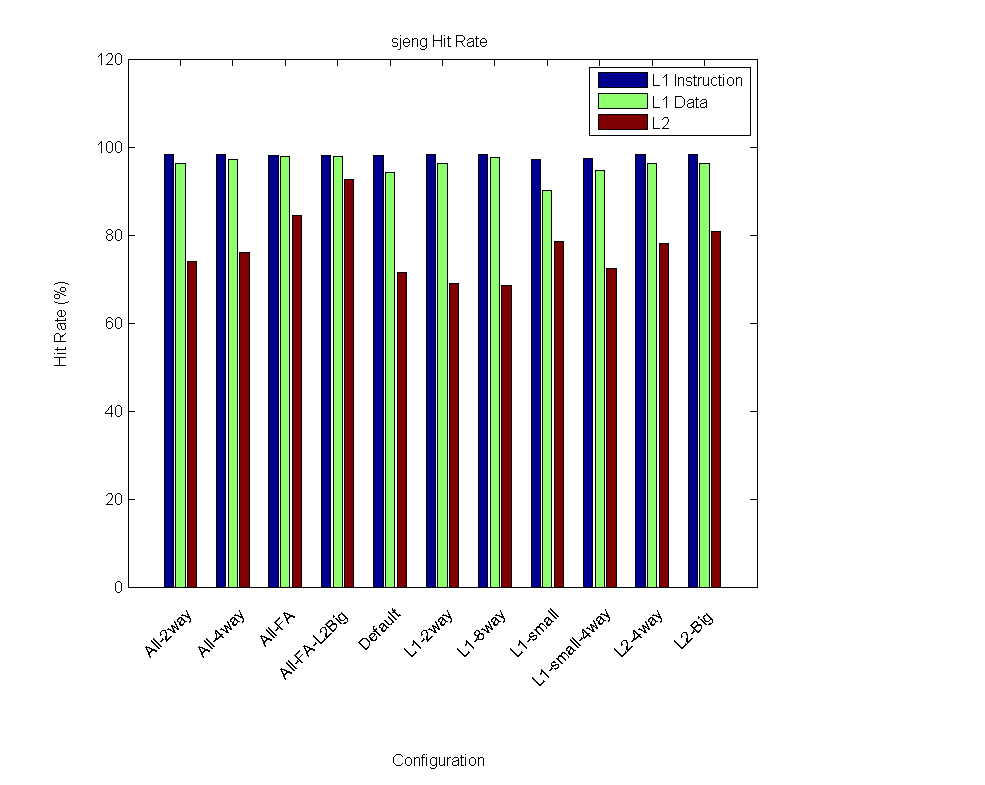
\includegraphics{hitRate_sjeng.png}

\hspace{-.9cm}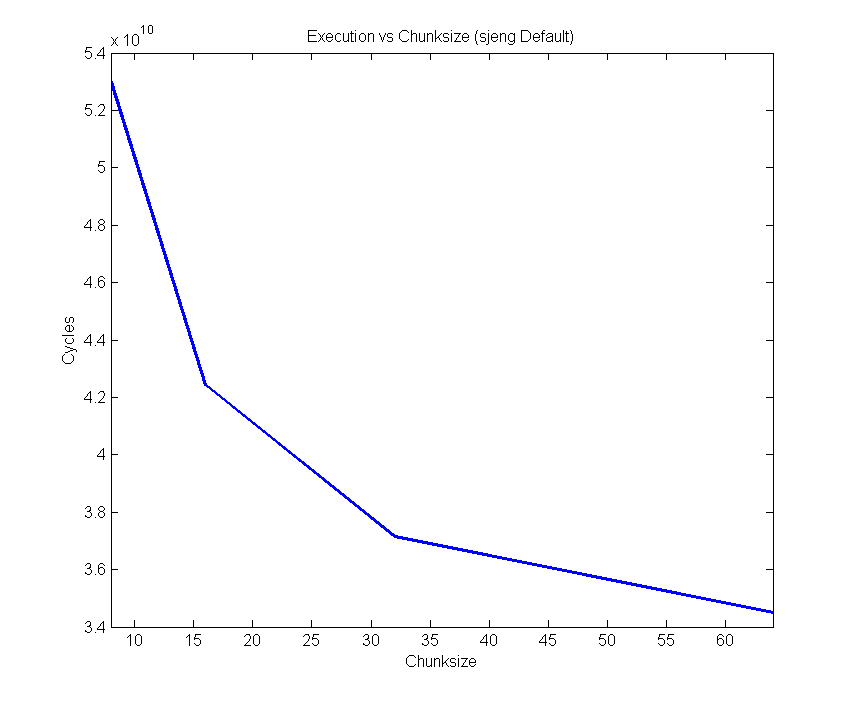
\includegraphics{chunksizeExecution.png}

\hspace{-.9cm}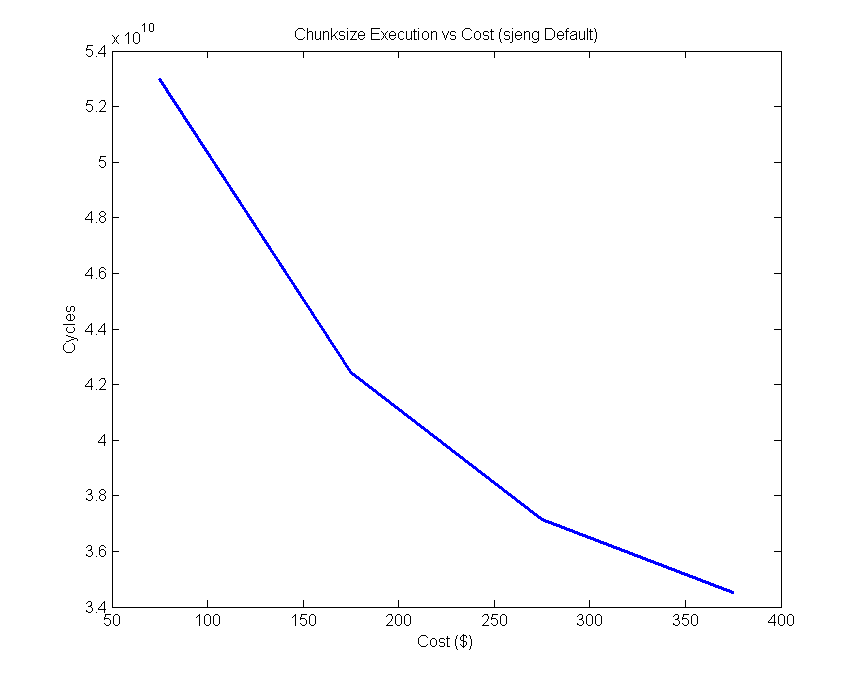
\includegraphics{chunksizeExecutionVsCost.png}


\end{document}